% !TeX root = main.tex
\documentclass[reprint,aps,unsortedaddress,superscriptaddress,prl,floatfix,showpacs,linenumbers]{revtex4-2}
\usepackage[utf8]{inputenc}
\usepackage{float}
\usepackage{graphicx}
\usepackage{amsmath,amsthm,amssymb}
\usepackage{verbatim}
\usepackage{url}
\usepackage{subcaption}
\usepackage[separate-uncertainty=true,range-units=single,range-phrase=\textendash]{siunitx}
\usepackage{physics}
\usepackage[pdfusetitle]{hyperref}
\usepackage[capitalize]{cleveref}
\usepackage[obeyFinal]{todonotes}
\setuptodonotes{inline}
\usepackage{adjustbox}
\usepackage{multirow}
\usepackage{lineno}
\usepackage{cmap}
\usepackage[version=4]{mhchem}
\usepackage{makecell}
\usepackage{comment}
\usepackage{orcidlink}
\usepackage{diagbox}
\linenumbers
\graphicspath{{figures/}}
\DeclareSIUnit\barn{b}

\pdfstringdefDisableCommands{%
  \def\,{}%
  \def\fnref#1{}%
}

\captionsetup{justification=raggedright,singlelinecheck=false}

\usepackage[most]{tcolorbox}

%\let\includegraphicsold\includegraphics
%\renewcommand{\includegraphics}[2][]{\tcbox{\includegraphicsold[#1]{#2}}}

\begin{document}

\title{Final SeaQuest results on the flavor asymmetry of the proton light-quark sea with proton-induced Drell-Yan process}
% !TeX root = main.tex
\author{C.~H.~Leung}
\affiliation{Department of Physics, University of Illinois at Urbana-Champaign, Urbana, Illinois 61801, USA}

\author{J.~C.~Peng}
\affiliation{Department of Physics, University of Illinois at Urbana-Champaign,
Urbana, Illinois 61801, USA}

\begin{comment}
\author{J. Dove}
\affiliation{Department of Physics, University of Illinois at Urbana-Champaign,
Urbana, Illinois 61801, USA}

\author{B.~Kerns}
\affiliation{Department of Physics, University of Illinois at Urbana-Champaign,
Urbana, Illinois 61801, USA}

\author{R.~E.~McClellan}
\altaffiliation[Present address ]{Pensacola State College, Pensacola, FL 32504}
\affiliation{Department of Physics, University of Illinois at Urbana-Champaign, 
Urbana, Illinois 61801, USA}

\author{S.~Miyasaka}
\affiliation{Department of Physics, Tokyo Institute of Technology, Meguro-ku, Tokyo 152-8550, Japan}

\author{D.~H.~Morton}
\affiliation{Randall Laboratory of Physics, University of Michigan, Ann Arbor,
Michigan 48109, USA}

\author{K.~Nagai}
\affiliation{Department of Physics, Tokyo Institute of Technology, Meguro-ku, Tokyo 152-8550, Japan}
\affiliation{Institute of Physics, Academia Sinica, Taipei, 11529, Taiwan}
\affiliation{Physics Division, Los Alamos National Laboratory, Los Alamos, New Mexico 97545, USA}

\author{S.~Prasad}
\affiliation{Department of Physics, University of Illinois at Urbana-Champaign,
Urbana, Illinois 61801, USA}
\affiliation{Physics Division, Argonne National Laboratory, Lemont, Illinois 60439, USA}

\author{F.~Sanftl}
\affiliation{Department of Physics, Tokyo Institute of Technology, Meguro-ku,
Tokyo 152-8550, Japan}

\author{M.~B.~C.~Scott}
\affiliation{Randall Laboratory of Physics, University of Michigan, Ann Arbor,Michigan 48109, USA}
\affiliation{Physics Division, Argonne National Laboratory, Lemont, Illinois 60439, USA}

\author{A.~S.~Tadepalli}
\altaffiliation[Present address ]{Thomas Jefferson National Accelerator Facility, Newport News, Virginia 23606, USA}
\affiliation{Department of Physics and Astronomy, Rutgers, The State University of New Jersey, Piscataway, New Jersey 08854, USA}

\author{C.~A.~Aidala}
\affiliation{Randall Laboratory of Physics, University of Michigan, Ann Arbor, Michigan 48109, USA}
\affiliation{Physics Division, Los Alamos National Laboratory, Los Alamos, New Mexico 87545, USA}

\author{J.~ Arrington}
\altaffiliation[Present address ]{Lawrence Berkeley National Laboratory, Berkeley, California, 94720 USA}
\affiliation{Physics Division, Argonne National Laboratory, Lemont, Illinois 60439, USA}

\author{C.~Ayuso}
\affiliation{Randall Laboratory of Physics, University of Michigan, Ann Arbor,
Michigan 48109, USA}

\author{C.~T.~Barker}
\affiliation{Department of Engineering and Physics, Abilene Christian University, Abilene, Texas 79699, USA}

\author{C.~N.~Brown}
\affiliation{Fermi National Accelerator Laboratory, Batavia, Illinois 60510, USA}

\author{T.~H.~Chang}
\affiliation{Institute of Physics, Academia Sinica, Taipei, 11529, Taiwan}

\author{W.~C.~Chang}
\affiliation{Institute of Physics, Academia Sinica, Taipei, 11529, Taiwan}

\author{A.~Chen}
\affiliation{Department of Physics, University of Illinois at Urbana-Champaign, Urbana, Illinois 61801, USA}
\affiliation{Institute of Physics, Academia Sinica, Taipei, 11529, Taiwan}
\affiliation{Randall Laboratory of Physics, University of Michigan, Ann Arbor, Michigan 48109, USA}

\author{D.~C.~Christian}
\affiliation{Fermi National Accelerator Laboratory, Batavia, Illinois 60510, USA}

\author{B.~P.~Dannowitz}
\affiliation{Department of Physics, University of Illinois at Urbana-Champaign, Urbana, Illinois 61801, USA}

\author{M.~Daugherity}
\affiliation{Department of Engineering and Physics, Abilene Christian University, Abilene, Texas 79699, USA}

\author{M.~Diefenthaler}
\affiliation{Department of Physics, University of Illinois at Urbana-Champaign, Urbana, Illinois 61801, USA}

\author{L.~El Fassi}
\affiliation{Department of Physics and Astronomy, Mississippi State University, Mississippi State, Mississippi 39762, USA }
\affiliation{Department of Physics and Astronomy, Rutgers, The State University of New Jersey, Piscataway, New Jersey 08854, USA}

\author{D.~F.~Geesaman}
\affiliation{Physics Division, Argonne National Laboratory, Lemont, Illinois 60439, USA}

\author{R.~Gilman}
\affiliation{Department of Physics and Astronomy, Rutgers, The State University of New Jersey, Piscataway, New Jersey 08854, USA}

\author{Y.~Goto}
\affiliation{RIKEN Nishina Center for Accelerator-Based Science, Wako, Saitama 351-0198, Japan}

\author{L.~Guo}
\altaffiliation[Present address ]{Florida International University, Miami, Florida, 33199, USA}
\affiliation{Physics Division, Los Alamos National Laboratory, Los Alamos, New Mexico 87545, USA}

\author{R.~Guo}
\affiliation{Department of Physics, National Kaohsiung Normal University, Kaohsiung City 80201, Taiwan}

\author{T.~J.~Hague}
\altaffiliation[Present address ]{Lawrence Berkeley National Laboratory, Berkeley, California, 94720 USA}
\affiliation{Department of Engineering and Physics, Abilene Christian University, Abilene, Texas 79699, USA}

\author{R.~J.~Holt}
\altaffiliation[Present address ]{Kellogg Radiation Laboratory, California Institute of Technology, Pasadena, California 91125, USA}
\affiliation{Physics Division, Argonne National Laboratory, Lemont, Illinois 60439, USA}

\author{D.~Isenhower}
\affiliation{Department of Engineering and Physics, Abilene Christian University, Abilene, Texas 79699, USA}

\author{E.~R.~Kinney}
\affiliation{Department of Physics, University of Colorado, Boulder,
Colorado 80309, USA}

\author{N.~D.~Kitts}
\affiliation{Department of Engineering and Physics, Abilene Christian University, Abilene, Texas 79699, USA}

\author{A.~Klein}
\affiliation{Physics Division, Los Alamos National Laboratory, Los Alamos, New Mexico 87545, USA}

\author{D.~W.~Kleinjan}
\affiliation{Physics Division, Los Alamos National Laboratory, Los Alamos, New Mexico 87545, USA}

\author{Y.~Kudo}
\affiliation{Department of Physics, Yamagata University, Yamagata City, Yamagata 990-8560, Japan}

\author{P.-J.~Lin}
\affiliation{Department of Physics, University of Colorado, Boulder, Colorado 80309, USA}
\affiliation{Institute of Physics, Academia Sinica, Taipei, 11529, Taiwan}

\author{K.~Liu}
\affiliation{Physics Division, Los Alamos National Laboratory, Los Alamos, New Mexico 87545, USA}

\author{M.~X.~Liu}
\affiliation{Physics Division, Los Alamos National Laboratory, Los Alamos,
New Mexico 87545, USA}

\author{W.~Lorenzon}
\affiliation{Randall Laboratory of Physics, University of Michigan, Ann Arbor,
Michigan 48109, USA}

\author{N.~C.~R.~Makins}
\affiliation{Department of Physics, University of Illinois at Urbana-Champaign, Urbana, Illinois 61801, USA}

\author{M.~Mesquita de Medeiros}
\affiliation{Physics Division, Argonne National Laboratory, Lemont,
Illinois 60439, USA}

\author{P.~L.~McGaughey}
\affiliation{Physics Division, Los Alamos National Laboratory, Los Alamos,
New Mexico 87545, USA}

\author{Y.~Miyachi}
\affiliation{Department of Physics, Yamagata University, Yamagata City,
Yamagata 990-8560, Japan}

\author{I.~Mooney}
\altaffiliation[Present address ]{Wayne State University, Detroit, MI 48202, USA}
\affiliation{Randall Laboratory of Physics, University of Michigan, Ann Arbor, Michigan 48109, USA}

\author{K.~Nakahara}
\altaffiliation[Present address ]{Stanford Linear Accelerator Center, Menlo Park, CA 94025, USA}
\affiliation{Department of Physics, University of Maryland, College Park, Maryland 20742, USA}

\author{K.~Nakano}
\affiliation{University of Virginia, Charlottesville, Virginia 22904, USA}
\affiliation{Department of Physics, Tokyo Institute of Technology, Meguro-ku, Tokyo 152-8550, Japan}
\affiliation{RIKEN Nishina Center for Accelerator-Based Science, Wako, Saitama 351-0198, Japan}

\author{S.~Nara}
\affiliation{Department of Physics, Yamagata University, Yamagata City, Yamagata 990-8560, Japan}


\author{A.~J.~Puckett}
\altaffiliation[Present address ]{University of Connecticut, Storrs, CT 06269, USA}
\affiliation{Physics Division, Los Alamos National Laboratory, Los Alamos, New Mexico 87545, USA}

\author{B.~J.~Ramson}
\affiliation{Randall Laboratory of Physics, University of Michigan, Ann Arbor, Michigan 48109, USA}
\affiliation{Fermi National Accelerator Laboratory, Batavia, Illinois 60510, USA}

\author{P.~E.~Reimer}
\affiliation{Physics Division, Argonne National Laboratory, Lemont, Illinois 60439, USA}

\author{J.~G.~Rubin}
\affiliation{Randall Laboratory of Physics, University of Michigan, Ann Arbor, Michigan 48109, USA}
\affiliation{Physics Division, Argonne National Laboratory, Lemont, Illinois 60439, USA}

\author{S.~Sawada}
\affiliation{Institute of Particle and Nuclear Studies, KEK, High Energy Accelerator Research Organization, Tsukuba, Ibaraki 305-0801, Japan}

\author{T.~Sawada}
\altaffiliation[Present address ]{Nambu Yoichiro Institute of Theoretical and Experimental Physics, Osaka Metropolitan University, Osaka 558-8585, JAPAN}
\affiliation{Randall Laboratory of Physics, University of Michigan, Ann Arbor, Michigan 48109, USA}

\author{T.-A.~Shibata}
\altaffiliation[Present address ]{Nihon University, College of Science and Technology, Chiyoda-ku, Tokyo 101-8308, Japan}
\affiliation{Department of Physics, Tokyo Institute of Technology, Meguro-ku, Tokyo 152-8550, Japan}
\affiliation{RIKEN Nishina Center for Accelerator-Based Science, Wako, Saitama 351-0198, Japan}

\author{S.~H.~Shiu}
\affiliation{Institute of Physics, Academia Sinica, Taipei, 11529, Taiwan}

\author{D.~Su}
\affiliation{Institute of Physics, Academia Sinica, Taipei, 11529, Taiwan}

\author{M.~Teo}
\affiliation{Department of Physics, University of Illinois at Urbana-Champaign, Urbana, Illinois 61801, USA}

\author{B.~G Tice}
\affiliation{Physics Division, Argonne National Laboratory, Lemont, Illinois 60439, USA}

\author{R.~S.~Towell}
\affiliation{Department of Engineering and Physics, Abilene Christian University, Abilene, Texas 79699, USA}

\author{S.~Uemura}
\altaffiliation[Present address ]{Fermi National Accelerator Laboratory, Batavia, Illinois 60510, USA}
\affiliation{Department of Engineering and Physics, Abilene Christian University, Abilene, Texas 79699, USA}

\author{T.~S.~Watson}
\affiliation{Department of Engineering and Physics, Abilene Christian University, Abilene, Texas 79699, USA}

\author{S.~G.~Wang}
\altaffiliation[Present address ]{APS, Argonne National Laboratory, Lemont, Illinois 60439, USA}
\affiliation{Institute of Physics, Academia Sinica, Taipei, 11529, Taiwan}
\affiliation{Department of Physics, National Kaohsiung Normal University, Kaohsiung City 80201, Taiwan}

\author{A.~B.~Wickes}
\affiliation{Physics Division, Los Alamos National Laboratory, Los Alamos,
New Mexico 87545, USA}

\author{J.~Wu}
\affiliation{Fermi National Accelerator Laboratory, Batavia, Illinois 60510, USA}

\author{Z.~Xi}
\affiliation{Department of Engineering and Physics, Abilene Christian University, Abilene, Texas 79699, USA}

\author{Z.~Ye}
\altaffiliation[Present address ]{Department of Physics, Tsinghua University, Beijing 100084 China}
\affiliation{Physics Division, Argonne National Laboratory, Lemont, Illinois 60439, USA}
\end{comment}
\author{Others...}
\collaboration{FNAL E906/SeaQuest Collaboration}
%\noaffiliation


\date{\today}

\begin{abstract}
	The Fermilab E906/SeaQuest collaboration performed measurements of the Drell-Yan process using
	\SI{120}{\GeV} proton beams bombarding liquid hydrogen and liquid deuterium targets.
	We performed a combined analysis of all collected data for the final results on the ratio of the $\sigma_{pd}/2\sigma_{pp}$ Drell-Yan cross
	section ratios covering the kinematic region of $0.13 < x < 0.45$.
	The $x$-dependencies of the $\bar{d}\left(x\right) / \bar{u}\left(x\right)$ and $\bar{d}\left(x\right) - \bar{u}\left(x\right)$
	are extracted from these cross section ratios.
	The $\bar{d}\left(x\right)$ is found to be greater than $\bar{u}\left(x\right)$ for the entire measured $x$
	range with improved statistical accuracy over previous measurements.
	The new results on $\bar{d}\left(x\right) / \bar{u}\left(x\right)$ and $\bar{d}\left(x\right) - \bar{u}\left(x\right)$
	are compared with various parton distribution functions and theoretical calculations.
\end{abstract}


\maketitle

%\section{Introduction}

Following the discovery of the point-like constituents in the proton in
deep-inelastic scattering (DIS) experiments, evidence for a nucleon sea,
made of quark-antiquark pairs,
was revealed from the observation of the sharp rise of the structure
functions as $x \to 0$. In contrast to the situation for atoms, where
the particle-antiparticle pairs play a relatively minor role, the
quark-antiquark pairs in the nucleon form an integral part for
depicting the internal structure of hadrons, owing to the large
coupling strength $\alpha_s$ in strong interactions~\cite{friedman1972}.

The earliest parton models assumed that the proton sea was SU(2)
flavor symmetric, even though proton's valence quark
distributions are not flavor symmetric. This flavor symmetry assumption
for the proton sea was not based on any known physics, instead reflecting the
expectation from perturbative QCD that the splitting of gluons
into quark-antiquark pairs should be nearly up-down flavor symmetric
due to the comparable masses for the up and down quarks.

Evidence for the asymmetry of the $\bar{u}$ and $\bar{d}$ sea-quark
distributions in the proton was first found in
deep inelastic scattering experiments~\cite{stein1975,amaudruz1991} via
the observation of the violation
of the Gottfried Sum Rule~\cite{gottfried1967}. Feynman and Field
attributed the asymmetry observed in the early SLAC DIS data to the Pauli
Exclusion Principle~\cite{field1977}. It was pointed out~\cite{ellis1991}
that an independent experimental technique to probe this flavor asymmetry is
to measure the Drell-Yan cross section ratios,
$\sigma_{pd}/2\sigma_{pp}$, which can further determine the $x$ dependence
of this flavor asymmetry.

The Drell-Yan cross section ratios,
$\sigma_{pd}/2\sigma_{pp}$, have been measured by the CERN NA51 experiment at
\SI{400}{\GeV} for a single value of $x$~\cite{NA51:1994xrz}, and by the FNAL
E866/NuSea experiment for the $0.015 < x < 0.35$ region with a \SI{800}{\GeV}
proton beam~\cite{hawker1998,peng1998,towell2001}. Subsequent measurements by the
HERMES collaboration, using the semi-inclusive DIS reaction~\cite{ackerstaff1998},
and by the STAR collaboration, using $W$-boson production in $p+p$ collision,
gave further confirmation of the up-down sea-quark flavor asymmetry in
the small $x$ region. The surprisingly large flavor asymmetry of the nucleon
sea has inspired much theoretical work discussed in several review
articles~\cite{kumano1998,vogt2000a,garvey2001,chang2014,geesaman2019}.

While the small $x$ region of the sea-quark flavor asymmetry was accurately
measured by the FNAL E866/NuSea experiment, the highest $x$ data points from
E866 suggest a possible reversal of the sea-quark flavor asymmetry for $x > 0.25$,
but with large statistical uncertainties. A new measurement with improved
accuracy for the large $x$ region was clearly warranted. The FNAL
E906/SeaQuest experiment, using a new spectrometer~\cite{aidala2019} and
a \SI{120}{\GeV} proton beam, was performed to shed new light on the flavor asymmetry
of the proton at the large $x$ region.

Results from the analysis of the first part of the SeaQuest data, corresponding
to roughly half of total data collected in the experiment, have been reported
in earlier publications~\cite{dove2021,dove2023}.
These analyses, adopting two different methods, showed that the
$\sigma_{pd}/2\sigma_{pp}$ Drell-Yan cross section ratios remain
above unity, implying that
$\bar{d}$ is greater than $\bar{u}$ for the entire $x$ range measured
at SeaQuest. Results on the $\sigma_{pd}/2\sigma_{pp}$  cross section ratios
for charmonium production, reported recently in
Ref.~\cite{leung2024a}, are also consistent with the flavor asymmetry
deduced from the Drell-Yan data.
Several recent global parton distribution function(PDF)
analyses~\cite{cocuzza2021,ball2022a,accardi2023,alekhin2023}
have included these results, in addition to the $W$ boson production data
from the STAR collaboration~\cite{adam2021}, to better constrain the
flavor asymmetry of $\bar u$ and $\bar d$ in the proton. The SeaQuest
flavor asymmetry data have also been compared the predictions from the
statistical model~\cite{soffer2019} and pion-cloud model~\cite{alberg2022}.

In this paper, we report the final results on the Drell-Yan measurements,
including all data sets collected by the SeaQuest experiment.
The data constitute a two-fold increase in the detected muons compared
to our previous publications. As the trigger
conditions and the detector configuration for the first and second parts
of the data sets are not
identical, the analysis was performed separately for each part of the
data sets.
Results obtained from the two data sets are first compared to check their
consistency, and then combined for the final results.
The results from the two data sets, except for the smallest $x_2$ point, are found to in good agreement,
with differences less than $1\sigma$.
The flavor asymmetry is very well constrained for the smallest $x_2$ bin by previous experiments,
and the final result on the measured cross section at the smallest $x_2$ bin is in better agreement
with theory expectation than the individual data set.

The SeaQuest experiment detects $\mu^+\mu^-$ pairs (dimuons) produced in
the interaction of a proton beam with various targets nuclei. The production
of massive dimuon pairs are described by the Drell-Yan
process~\cite{drell1970} with the leading order (LO) cross section given as
\begin{multline}
	\frac{d^2\sigma}{dx_1dx_2}=\frac{4\pi \alpha^2}{9x_1x_2s} \times
	\label{eq:DYCross} \\
	\sum_{i\in u,d,s,\dots} e_i^2 \left[q_i^A\left(x_1\right) \bar q_i^B\left(x_2\right) + \bar q_i^A\left(x_1\right)
		q_i^B\left(x_2\right)\right],
\end{multline}
where $\alpha$ is the fine-structure constant,
$s$ is the center-of-mass energy squared,
$e_i$ is the charge of a quark
with flavor $i$, and $q_i^{A,B}\left(x_{1,2}\right)$ are the quark
distribution functions in hadrons $A$ and $B$
for quarks carrying a momentum fraction $x_1$ and $x_2$, respectively.
An analogous notation is used for antiquark distribution functions
$\bar q_i^{A,B}\left(x_{1,2}\right)$.
For fixed-target experiments like SeaQuest, the spectrometers have
large acceptance only for the positive $x_F (x_F = x_1 - x_2)$ region. %Can we really say this?
Thus, the Drell-Yan cross section is dominated by
the first term, corresponding to the annihilation of a beam quark with
a target antiquark. Assuming
$\sigma^{pd} \approx \sigma^{pp} + \sigma^{pn}$,
which neglects small nuclear effects of the
deuteron~\cite{kumano1998,ehlers2014},
and charge symmetry for the parton distributions~\cite{londergan2010},
\cref{eq:DYCross} yields the following approximation for the target ratio:
\begin{equation}
	\begin{split}
		\frac{\sigma^{pd}}{2\sigma^{pp}} & \approx
		\frac{1}{2} \frac{4+\frac{d\left(x_1\right)}
			{u\left(x_1\right)}}{4+\frac{d\left(x_1\right)}
			{u\left(x_1\right)}\frac{\bar d\left(x_2\right)}{\bar u\left(x_2\right)}}
		\left[1+\frac{\bar d\left(x_2\right)}{\bar u\left(x_2\right)}\right]                         \\
		                                 & \approx \frac{1}{2} \left[1+\frac{\bar d\left(x_2\right)}
			{\bar u\left(x_2\right)}\right].
	\end{split}
	\label{eq:crRatio}
\end{equation}

While \cref{eq:crRatio} illustrates the power of the $\sigma^{pd}/2\sigma^{pp}$ Drell-Yan cross section
ratio to reveal the flavor asymmetry between $\bar{d}$ and $\bar{u}$,
the actual extraction of the $\bar{d}\left(x\right) / \bar{u}\left(x\right)$
ratios from the measured $\sigma^{pd}/ 2 \sigma^{pp}$ Drell-Yan cross
section ratios is performed using Next-to-Leading Order (NLO)
calculation.

The SeaQuest spectrometer is  described in detail in Ref.~\cite{aidala2019}.
The experiment receives the  proton beam from the Fermilab Main
Injector at \SI{120}{\GeV}
once every minute in 4-second periods (spills), with average intensity
of \num{6e12} per spill.
The target system consists of two liquid targets (hydrogen and deuterium),
three solid targets (iron, carbon and tungsten), and two calibration
targets (``empty flask'' and ``no target'').
A solid iron magnet focuses the high mass dimuons into the spectrometer.
The spectrometer consists of four tracking stations, with an open
air magnet between stations~1 and~2.
Each tracking station consists of hodoscope planes, which
provide fast signals for triggering,
and drift chambers or proportional tubes, which provide precise
position information for tracking.
The main physics trigger requires a coincidence of two opposite sign muons,
one in the top half and one in the bottom half of the spectrometer.
A separate trigger only requires one muon track, and it is mainly used
for studying the accidental background.

%\section{Data Analysis}
%\label{sec:analysis}
The muon tracks are reconstructed using the hits in the drift chambers and proportional tubes in each station.
After identifying hits potentially originating from interactions within the target region,
the Kalman filter algorithm~\cite{kalman1960} is used to reconstruct the muon tracks.
%and determine the best estimate of the muon momentum.
%The magnetic field of the two magnets and the energy loss in the solid iron FMag are also taken into account during this stage.
Pairs of oppositely charged muons tracks from the top and bottom sections of the spectrometer are
matched to determine the interaction vertex using the Kalman filter.
A detailed description of the analysis procedure can be found in earlier publication~\cite{dove2021,dove2023}.

\begin{figure}[htbp!]
	\centering
	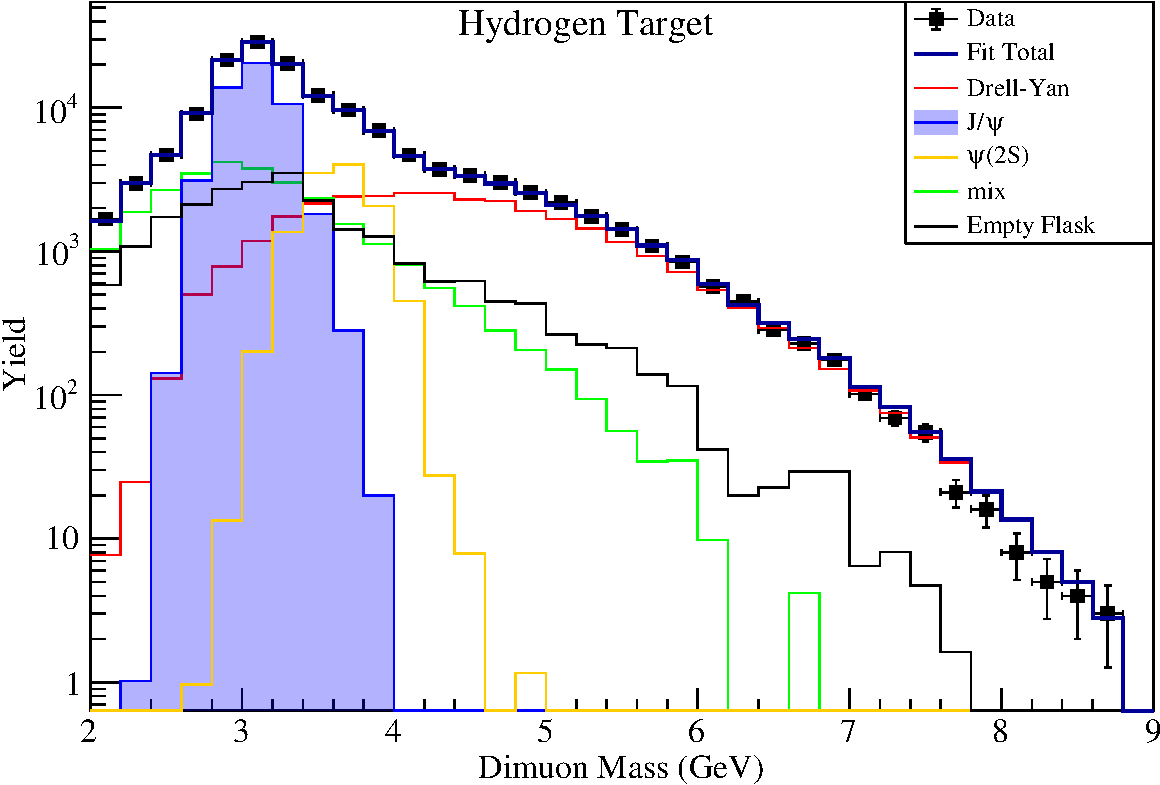
\includegraphics[width=\linewidth]{massfit_run56_LH2.pdf}
	\caption{Dimuon mass distribution for events collected
		on liquid hydrogen target for the second data set.
		The data points (solid squares) are compared with a fit consisting of
		various components (see text).}
	\label{fig:massfit}
\end{figure}

A GEANT4~\cite{agostinelli2003,allison2006,allison2016} based Monte
Carlo simulation has been developed to compare data with expectations.
%To compare the experimental results with theoretical expectations,
%a GEANT4~\cite{agostinelli2003,allison2006,allison2016} based Monte Carlo simulations has been developed.
The Drell-Yan events are generated with the dimuon mass and $x_F$
distributions obtained with the CT14 nucleon PDFs~\cite{hou2018}.
The dimuon transverse momentum distribution is adjusted to match the measured distribution~\cite{prasad2020,leung2024}.
%Other PDFs, such as the statistical model~\cite{soffer2019}, were used to measure the systematic effects due to input PDFs.
The efficiency and the resolution of the chambers are taken into account in the simulation.
%by dropping a small number of hits, and applying Gaussian smearing to the drift distance of the remaining hits.
%Both the efficiency and the width of the smearing are taken from the data.
An embedding procedure has also been developed to simulate the background hits by embedding each Monte Carlo event
with hits recorded by the random trigger~\cite{dove2020}.

The dimuon mass spectrum, as shown in \cref{fig:massfit} for data collected
on the liquid hydrogen target for the second part of the experiment, consists
of various components including the Drell-Yan process, the charmonium
production, accidental background, and other background sources.
These different components often have distinct mass spectra, for example, the $J/\psi$
and $\psi\left(2S\right)$ decays would have sharp distributions centered around their masses.
Therefore, the data can be fitted to various templates to obtain
the relative contribution from each source.
As input parameters to the fit, the mass distributions for $J/\psi$, $\psi\left(2S\right)$
and the Drell-Yan are obtained from studying the Monte Carlo simulation. %, as discussed in \cref{subsec:MC}.
The mass distribution of accidental coincidence events was made by pairing at random $\mu^+$ and $\mu^-$ collected with the ``single-muon'' trigger
under the condition that the beam intensities of $\mu^+$ and $\mu^-$ events were comparable.
The magnitudes of these components,
with the exception of the empty-flask data for which the normalization is known,
were varied in the fit to the mass spectrum.
The statistical uncertainties of the Monte Carlo and empty-flask date are taken into account using the algorithm described in Ref.~\cite{barlow1993}.
\Cref{fig:massfit} shows the fit to the $p+p$ dimuon spectrum,
and the mass distribution is well described by this fitting procedure.

After the mass fit is performed,
a mass cut ($M>\SI{4.5}{\GeV}$) is applied to remove the $J/\psi$ and $\psi\left(2S\right)$ events.
The remaining events are projected into various kinematic variables, such as $x_1$, $x_2$, $x_F$, and $P_T$.
The accidental background and empty-flask contributions are then subtracted from the data.
Several corrections are applied to extract the final Drell-Yan yields.
These include the deadtime correction for the effective luminosity,
a target contamination correction is also applied for the \ce{D_2} data due to \ce{H} contamination in the target cell.
The reconstruction inefficiency and data acquisition system deadtime, which have a small but non-negligible target dependence,
are also taken into account.
For this analysis,
a revised target contamination correction is used as compared with the earlier work~\cite{dove2021,dove2023},
resulting in a roughly \SI{2}{\percent} shift in the measured cross section ratios.

\begin{table*}[htbp!]
	\centering
	\caption{The measured $\sigma_{pd}/2\sigma_{pp}$ cross section ratio as well
		as the extracted $\bar{d}/\bar{u}$ and $\bar{d}-\bar{u}$ for each $x_{2}$ bin.
		The first uncertainty is statistical and the second systematic.
		The average values of kinematic variables in each $x_2$ bin are also shown.}
	\label{tab:dbarubar}
	\begin{adjustbox}{max width=\textwidth}
		% !TeX root = ../main.tex
{
\renewcommand{\arraystretch}{1.5}
\begin{tabular}{cccccccc}
	\hline\hline
	$x_{2}$ range    & $\expval{x_{2}}$ & $\expval{x_{1}}$ & $\expval{p_{T}}(\unit{\GeV/c})$ & $\expval{M}(\unit{\GeV/c^2})$ & $\sigma_{pd}/2\sigma_{pp}$ & $\bar{d}/\bar{u}$                     & $\bar{d}-\bar{u}$                     \\ \hline
	$0.130$--$0.160$ & $0.146$          & $0.687$          & $0.760$                         & $4.71$                        & $1.177\pm0.033\pm0.028$    & $1.383^{+0.058+0.060}_{-0.053-0.060}$ & $0.176^{+0.021+0.024}_{-0.022-0.023}$ \\
	$0.161$--$0.201$ & $0.181$          & $0.610$          & $0.759$                         & $4.87$                        & $1.174\pm0.022\pm0.025$    & $1.431^{+0.041+0.061}_{-0.051-0.061}$ & $0.111^{+0.011+0.011}_{-0.011-0.011}$ \\
	$0.202$--$0.242$ & $0.222$          & $0.553$          & $0.760$                         & $5.11$                        & $1.275\pm0.024\pm0.027$    & $1.672^{+0.052+0.082}_{-0.052-0.082}$ & $0.092^{+0.012+0.012}_{-0.012-0.012}$ \\
	$0.243$--$0.293$ & $0.263$          & $0.516$          & $0.761$                         & $5.44$                        & $1.232\pm0.029\pm0.037$    & $1.653^{+0.073+0.123}_{-0.073-0.113}$ & $0.043^{+0.003+0.013}_{-0.003-0.013}$ \\
	$0.294$--$0.354$ & $0.324$          & $0.492$          & $0.762$                         & $5.83$                        & $1.205\pm0.040\pm0.052$    & $1.694^{+0.124+0.174}_{-0.114-0.174}$ & $0.024^{+0.004+0.004}_{-0.004-0.004}$ \\
	$0.355$--$0.455$ & $0.395$          & $0.474$          & $0.762$                         & $6.34$                        & $1.212\pm0.055\pm0.047$    & $1.925^{+0.205+0.205}_{-0.195-0.205}$ & $0.015^{+0.005+0.005}_{-0.005-0.005}$ \\ \hline\hline
\end{tabular}
}

	\end{adjustbox}
\end{table*}

%\section{Measurement of The \texorpdfstring{$\sigma_{pd}/2\sigma_{pp}$}{pd/2pp} Drell-Yan Cross Section Ratio}
%\label{sec:csr}
The $\sigma_{pd}/2\sigma_{pp}$ cross
section ratios obtained from the analysis of the full SeaQuest
data set are shown in \Cref{fig:xT_csr}.
The main systematic uncertainties originate from the modeling of the
accidental background (\qtyrange{0.41}{3.82}{\percent}).
Different methods for generating the accidental background distributions
have been studied~\cite{pate2023} to estimate the uncertainty,
and the differences are quoted as the systematic uncertainty.
Other sources of systematic uncertainties include the efficiency
corrections (\qtyrange{0.46}{0.74}{\percent}),
empty flask normalization (\qtyrange{0.10}{0.16}{\percent}), and the
relative beam luminosity (\SI{2}{\percent}).

\begin{figure}[htbp!]
	\centering
	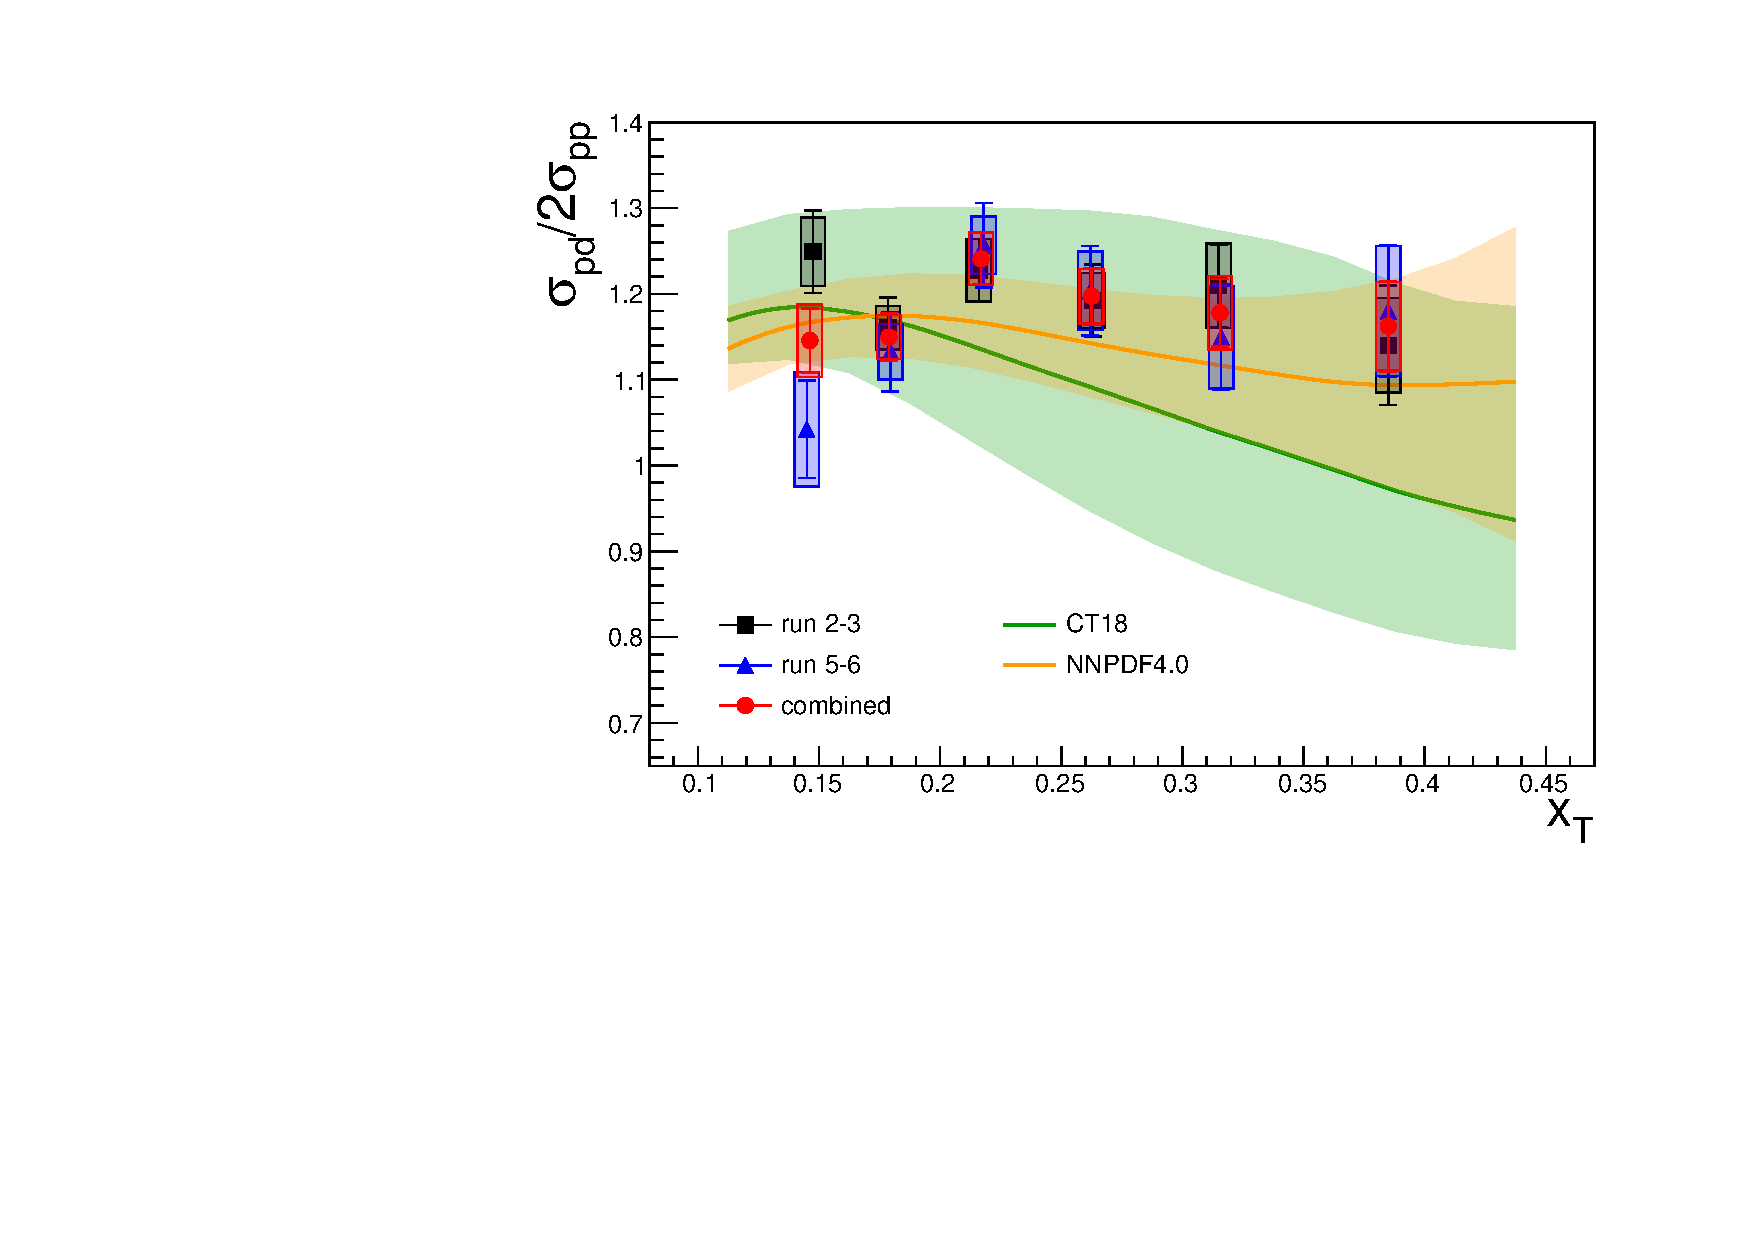
\includegraphics[width=\linewidth]{data_full_xT_syst.pdf}
	\caption{Measured $\sigma_{pd}/2\sigma_{pp}$ Drell-Yan cross section ratio from SeaQuest compared calculations using
		CJ15~\cite{accardi2016a}, CJ22~\cite{accardi2023}, and NNPDF4.0~\cite{ball2022a}.
		The error bands on the theoretical calculations correspond to the \SI{68}{\percent} confidence level from the PDFs.}
	\label{fig:xT_csr}
	%\todo{which PDFs to use?}
	%\todo[author=JCPeng,color=red]{use blue and red color for the part A and part B results.
	%Also, change Run 2-3 to Part A and Run 5-6 to Part B}
	%\todo{break this into mutliple figures. Some curves can be moved to the appendix.}
\end{figure}

%\todo{Update discussion here. Only the combined results are shown}
The two data sets are analyzed separately, and compared for consistency.
The final results are obtained by taking an average,
weighted by the inverse of the total uncertainty squared.
The results are shown in \Cref{fig:xT_csr} and tabulated in \cref{tab:dbarubar}.
\Cref{fig:xT_csr} compares the SeaQuest results with
NLO calculations using DYTurbo~\cite{camarda2020},
with nucleon PDFs CJ15~\cite{accardi2016a}, CJ22~\cite{accardi2023}, and NNPDF4.0~\cite{ball2022a}.
Note that CJ15 was obtained without input from the first
SeaQuest result~\cite{dove2021}, while the first SeaQuest result was included
in the global fit for CJ22 and NNPDF4.0. This accounts for the better agreement between
the data and the NNPDF4.0 calculation, although the data tend to be higher than
the calculation for the large $x$ region. 
Nevertheless, \Cref{fig:xT_csr}
shows that both the data and the NNPDF4.0 calculation for the
$\sigma_{pd}/2\sigma_{pp}$ cross section ratio are larger than unity for the
entire measured $x$ region.
Despite both including both including our earlier results,
CJ22 and NNPDF4.0 predicted different behavior for the $\sigma_{pd}/2\sigma_{pp}$ ratio.
With the increased statistics in the updated analysis,
the constrain on the light sea-quark asymmetry in future global analysis can be further improved. 


\begin{comment}
\begin{table}
	\centering
	\caption{Breakdown of systematic uncertainty for $\sigma_{pd}/2\sigma_{pp}$ ratio in each $x_2$ bins.}
	\label{tab:sys_csr}
	\begin{adjustbox}{max width=\linewidth}
		\input{table/DY-csr/MF-xT-new.tex}
	\end{adjustbox}
\end{table}
\end{comment}

To facilitate the comparison between SeaQuest result with predictions
from various models, the $\bar{d}(x)/\bar{u}(x)$ ratio is extracted from the
cross section ratio by an iterative method, as described in
Ref.~\cite{dove2021}.
We first estimate the $\bar{d}(x)/\bar{u}(x)$ ratio over the measured $x_2$
and calculate the cross section ratio $R$ using a chosen PDF set.
This PDF set provides all parton distributions including the
$\bar{d}(x)+\bar{u}(x)$, except that the $\bar{d}(x)/\bar{u}(x)$
ratios are allowed to vary.
The calculated cross section is weighted by the spectrometer acceptance calculated using Monte Carlo simulations.
The acceptance is tabulated in \cref{tab:acceptance}.
The cross section ratios $R$ are then calculated up to next-to-leading order
as a function of $x_2$ and compared with the data. The $\bar{d}(x)/\bar{u}(x)$
ratios are then adjusted until the difference between data and
calculation is less than $10^{-3}$.

\begin{figure*}[htpb!]
	\centering
	\begin{subfigure}{0.45\linewidth}
		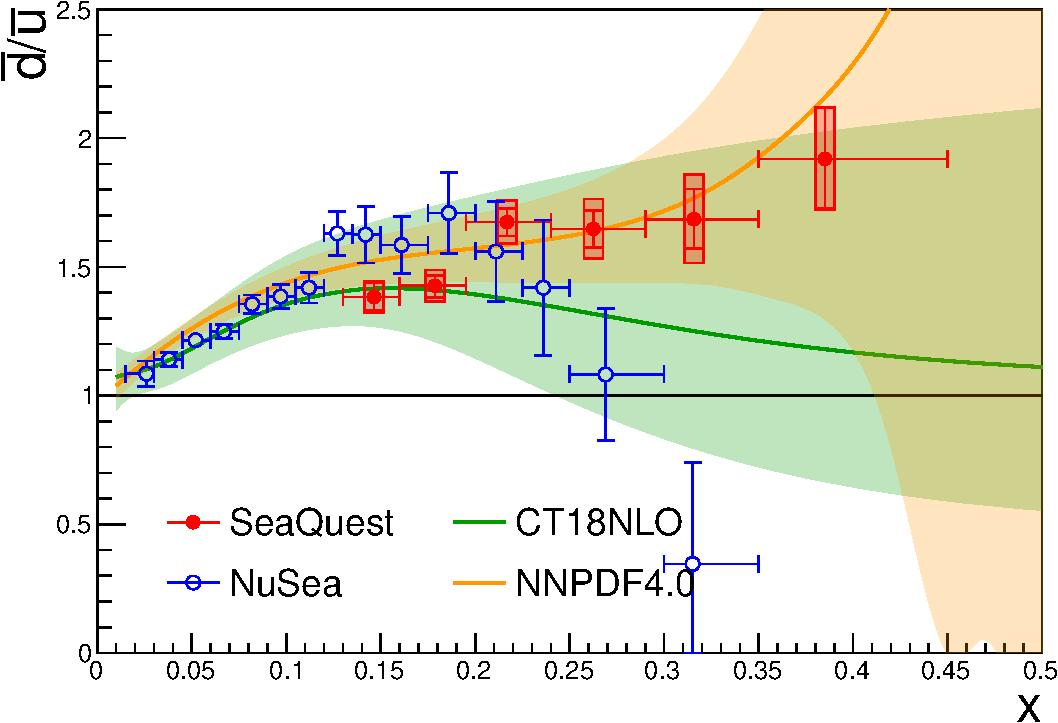
\includegraphics[width=\linewidth]{E906_E866_dbarubar_PDF.pdf}
	\end{subfigure}
	\begin{subfigure}{0.45\linewidth}
		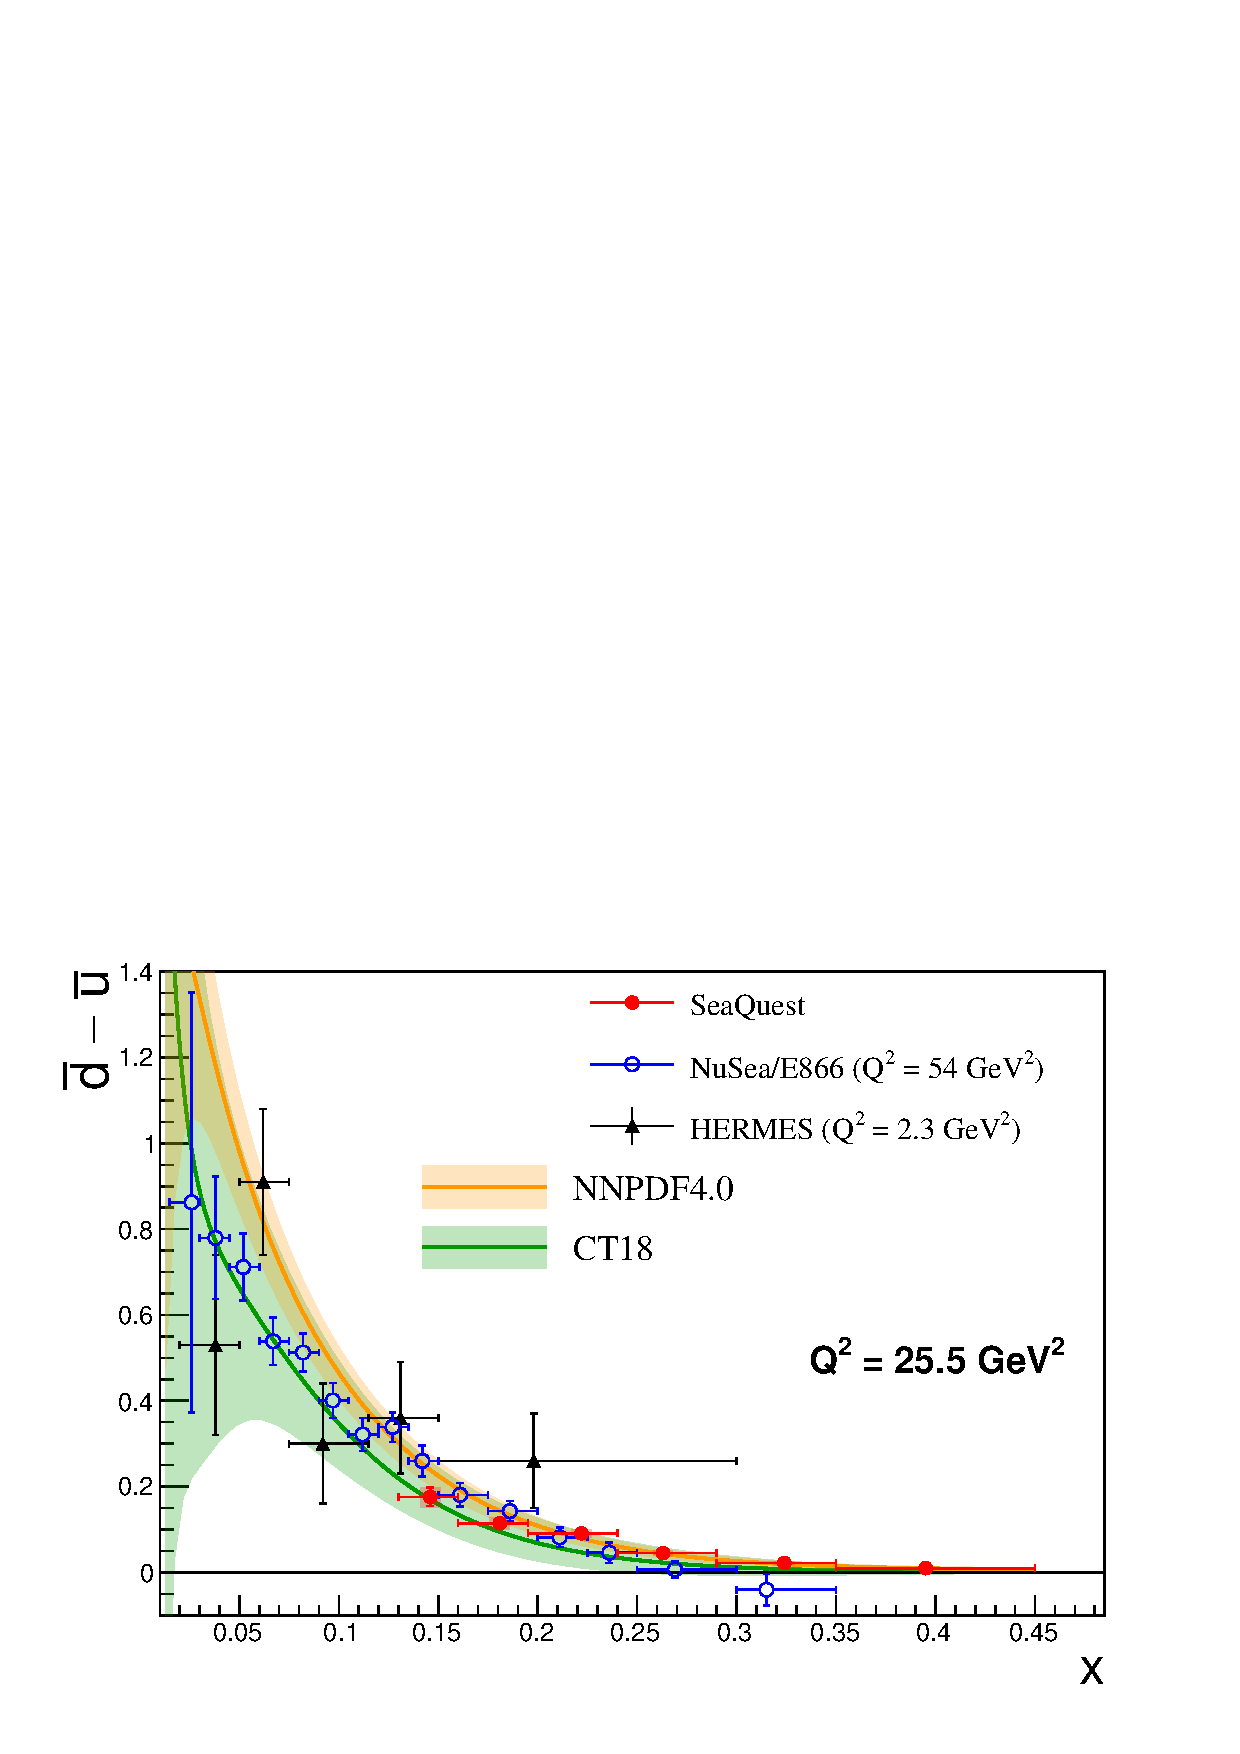
\includegraphics[width=\linewidth]{dbub_diff_with_PDF.pdf}
	\end{subfigure}
	\begin{subfigure}{0.45\linewidth}
		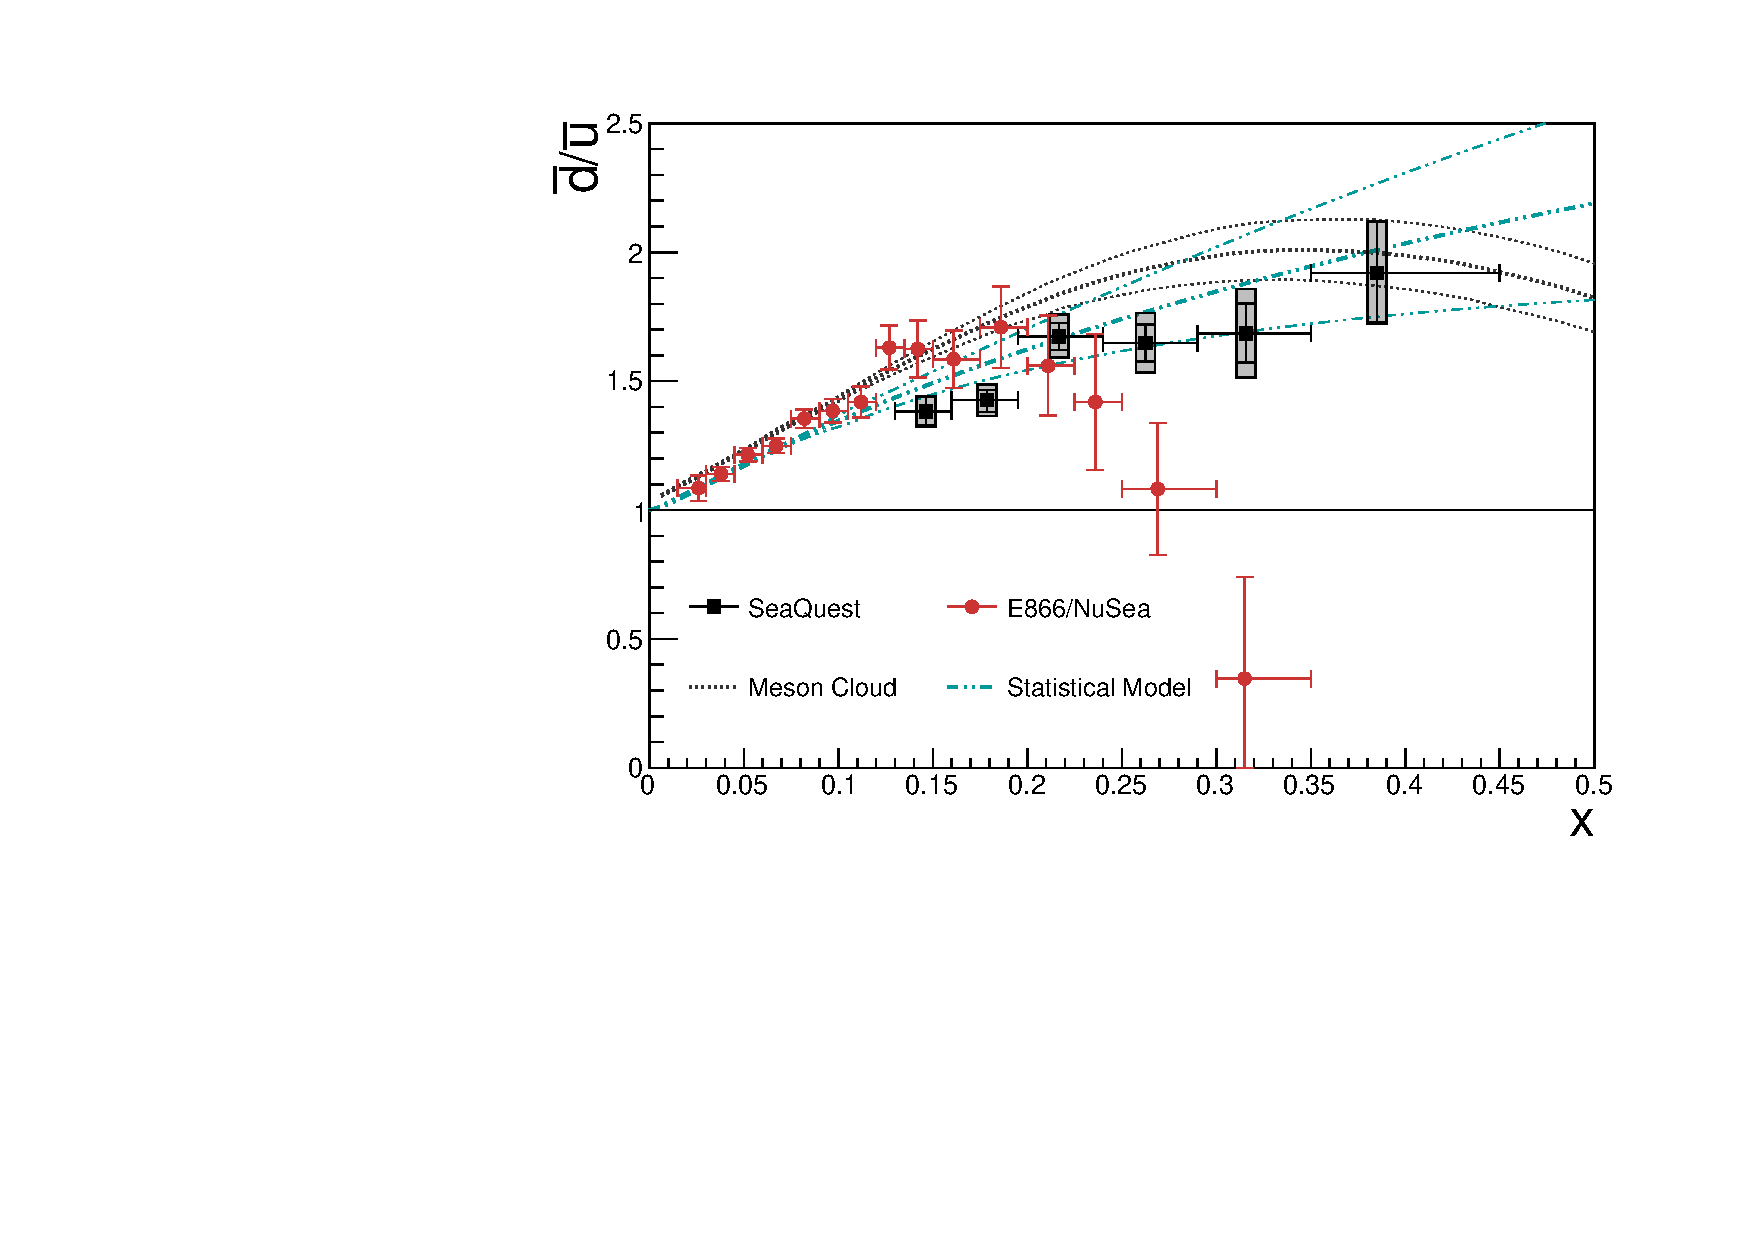
\includegraphics[width=\linewidth]{E906_E866_dbarubar_model.pdf}
	\end{subfigure}
	\begin{subfigure}{0.45\linewidth}
		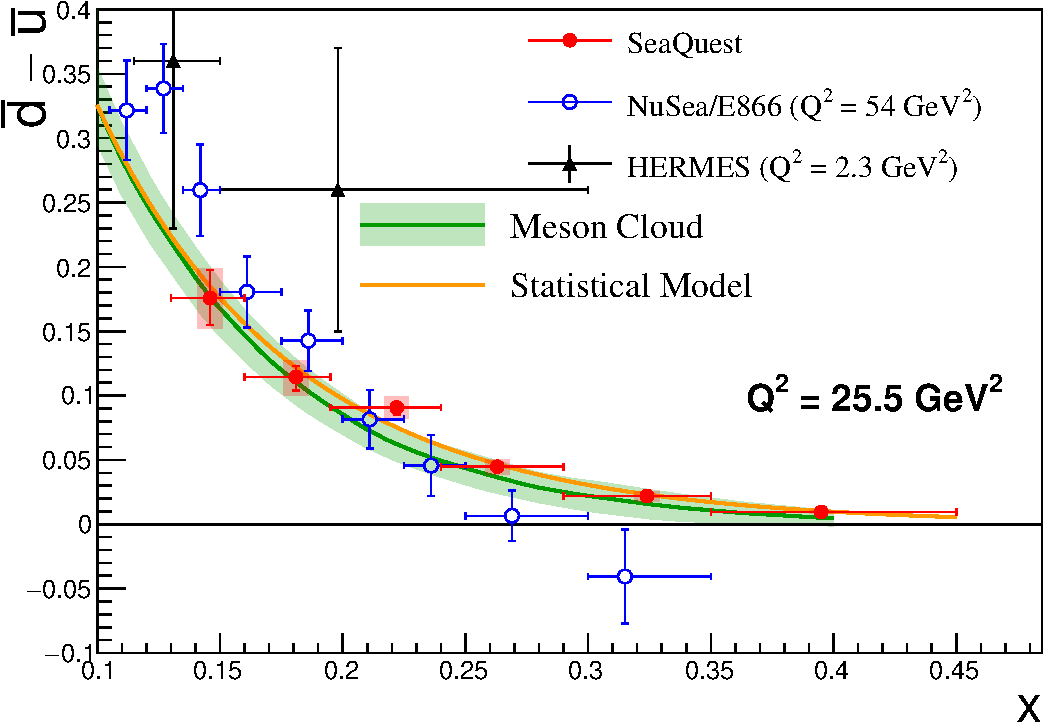
\includegraphics[width=\linewidth]{dbub_diff_with_model.pdf}
	\end{subfigure}
	\caption{The extracted $\bar{d}(x)/\bar{u}(x)$ (left) and $\bar{d}(x)-\bar{u}(x)$ (right)
		from the measured $\sigma_{pd}/2\sigma_{pp}$ Drell-Yan cross section ratio
		from SeaQuest (black square), E866~\cite{towell2001} (red circles), and HERMES~\cite{ackerstaff1998} (blue triangles).
		The extracted ratios are compared with CJ22~\cite{accardi2023}, and NNPDF4.0~\cite{ball2022a} global PDF analyses (top),
		and with predictions from meson cloud model~\cite{alberg2022} and statistical model~\cite{soffer2019} (bottom).
		The error bands on the PDFs correspond to their \SI{68}{\percent} confidence level.
	}
	\label{fig:e906_e866_dbarubar}
\end{figure*}

The extracted $\bar{d}(x)/\bar{u}(x)$ from the measured SeaQuest cross section ratio,
using the CT18 PDFs as the basis, are shown in \cref{fig:e906_e866_dbarubar}
and tabulated in \cref{tab:dbarubar}.
While the SeaQuest results are consistent with previous E866
results~\cite{towell2001} at low $x$,
the extracted $\bar{d}(x)/\bar{u}(x)$ ratios from the SeaQuest measurement
continue to rise as $x$ increases,
and is in tension with the E866 result.
The SeaQuest results are also in much better agreement with
predictions from the meson cloud model~\cite{alberg2022}
and the statistical model~\cite{soffer2019}.
The extracted $\bar{d}(x)/\bar{u}(x)$ ratios are also compared with results
from CJ22~\cite{accardi2023} and NNPDF4.0~\cite{ball2022a}
global analyses in \cref{fig:e906_e866_dbarubar}.
NNPDF4.0 and the CJ22 global analyses, which both include the earlier SeaQuest results~\cite{dove2021},
both prefer the $\bar{d}(x)/\bar{u}(x)>1$ in the large $x$ region covered by the SeaQuest measurement.
With the improved statistical accuracy from the combined analysis
presented in this paper, the uncertainty on the $\bar{d}(x)/\bar{u}(x)$ in
these global analyses can be further reduced.


\begin{table*}[htbp!]
	\centering
	\caption{Values of $\int_{0.45}^{0.13} \left[\bar{d}\left(x\right) - \bar{u}\left(x\right)\right] \dd{x}$
		and $\int_{0.45}^{0.13} x\left[\bar{d}\left(x\right) - \bar{u}\left(x\right)\right] \dd{x}$ at $Q^2=\SI{25.5}{\GeV\squared}$ extracted from
		SeaQuest compared with CJ15~\cite{accardi2016a}, CJ22~\cite{accardi2023}, NNPDF4.0~\cite{ball2022a}
		PDFs as well as the meson cloud~\cite{alberg2022} and the statistical models~\cite{soffer2019}.}
	\label{tab:dbarMubar}
	\begin{adjustbox}{max width=\linewidth}
		% !TeX root = ../main.tex
\renewcommand{\arraystretch}{1.5}
\begin{tabular}{ccccccc}
\hline \hline
 &          & \multicolumn{2}{c}{PDFs} & & \multicolumn{2}{c}{Models} \\ \cline{3-4} \cline{6-7}
 & SeaQuest &CJ22     & NNPDF4.0     & & Stat.     & Meson cloud    \\ \hline
$\int^{0.45}_{0.13} \left[\bar{d}\left(x\right) - \bar{u}\left(x\right) \right]\dd{x}$ &
  $0.0179_{-0.0018}^{+0.0017} {}_{-0.0023}^{+0.0022}$ &
  $0.0167^{+0.0009}_{-0.0028}$ &
  $0.0208^{+0.0036}_{-0.0036}$ & &
  $0.0186$ &
  $0.0180$ \\
$\int^{0.45}_{0.13} x\left[\bar{d}\left(x\right) - \bar{u}\left(x\right) \right]\dd{x}$ &
  $0.00368_{-0.00036}^{+0.00034} {}_{-0.00049}^{+0.00045}$ &
  $0.00319^{+0.00019}_{-0.00063}$ &
  $0.00414^{+0.00078}_{-0.00078}$ & &
  $0.00386$ &
  $0.00361$ \\ \hline \hline
\end{tabular}

	\end{adjustbox}
\end{table*}

The isovector quantity, $\bar{d}(x) - \bar{u}(x)$,
is of interest since the perturbative processes should not produce any significant difference between $\bar{d}(x)$ and $\bar{u}(x)$.
Hence, $\bar{d}(x) - \bar{u}(x)$ can provide a direct measure of the non-perturbative contribution to the proton sea.
%Moreover, recent advances in lattice QCD advances have enabled the calculation of $\bar{d}(x) - \bar{u}(x)$, to be compared with the data.
From the $\bar{d}(x) / \bar{u}(x)$ ratios extracted from SeaQuest,
we have calculated $\bar{d}(x) - \bar u(x)$ by taking the $\bar{d}(x) + \bar{u}(x)$ values from the CT18 proton PDFs.
The values of $\bar{d}(x)-\bar{u}(x)$ derived from the SeaQuest data are
shown in \cref{fig:e906_e866_dbarubar} and tabulated in \cref{tab:dbarubar},
and are compared with results from E866~\cite{towell2001} and
HERMES~\cite{ackerstaff1998}.
The derived $\bar{d}(x)-\bar{u}(x)$ are also compared with predictions from the meson cloud and the statistical models in \cref{fig:e906_e866_dbarubar}.
Like the $\bar{d}(x) / \bar{u}(x)$ ratio, the deduced $\bar{d}-\bar{u}$ is also in good agreement with both models.

The SeaQuest data can also be used to calculate two integrals:
$\int^{0.45}_{0.13} \left[\bar{d}\left(x\right) - \bar{u}\left(x\right) \right]\dd{x}$,
which describes the integrated sea-quark flavor asymmetry, and
$\int^{0.45}_{0.13} x\left[\bar{d}\left(x\right) - \bar{u}\left(x\right) \right]\dd{x}$,
which represents the difference in the momentum fractions carried
by $\bar{u}$ and $\bar{d}$ quarks.
These values are listed in \cref{tab:dbarMubar}, and compared with different PDFs and models.
The SeaQuest results are in good agreement with NNPDF4.0 and with the model predictions.

In summary, we have reported the improved results on the
$\sigma_{pd}/2\sigma_{pp}$ Drell-Yen cross section ratio up to $x_2=0.45$,
based on the analysis of the entire SeaQuest dataset,
which supersedes the earlier results in Ref.~\cite{dove2021,dove2023}.
The measured ratio remains above unity,
which suggests the $\bar{d}(x)/\bar{u}(x)$ ratio continues to increase at large $x$.
The improved statistical precision presented in this paper will help to
further constrain the light sea-quark asymmetry in future global analysis.
These results support the excess of $\bar{d}$ compared to $\bar{u}$ that is obtained in various model predictions,
including the meson cloud model and the statistical model.
With recent developments in lattice calculations within the framework
of large momentum effective theory~\cite{constantinou2021},
these results can provide an important benchmark for the lattice
calculations in the future.
With the advent of the Electron Ion Collider, the flavor asymmetry in the small $x$ region,
where abundant sea-quarks reside, can be further measured via the semi-inclusive DIS reaction~\cite{ackerstaff1998}.

\begin{acknowledgments}
	This work was performed by the SeaQuest Collaboration, whose work was supported in part by the
	\todo{Add funding information.}
\end{acknowledgments}
\bibliography{reference}

\appendix
\section{End Matter}
\begin{table*}[htbp]
	\centering
	\caption{The acceptance of the spectrometer for different $x_1$ and $x_2$ bins.
		In each cell, the first value is the acceptance,
		the second is the average $x_1$, the third is the average $x_2$,
		and the fourth is the average mass in \unit{\GeV/c^2}.}
	\label{tab:acceptance}
	\begin{adjustbox}{max width=\linewidth}
		\begin{tabular}{c|c|c|c|c|c|c|c|c|c|c}
			\hline
			\hline
			\diagbox{$x_2$}{$x_1$} & $0.30$--$0.35$                                                           & $0.35$--$0.40$                                                           & $0.40$--$0.45$                                                           & $0.45$--$0.50$                                                           & $0.50$--$0.55$                                                           & $0.55$--$0.60$                                                           & $0.60$--$0.65$                                                           & $0.65$--$0.70$                                                           & $0.70$--$0.75$                                                           & $0.75$--$0.80$                                                           \\
			\hline
			$0.130$--$0.160$       &                                                                          &                                                                          &                                                                          &                                                                          &                                                                          & \begin{tabular}{@{}c@{}} $1.19\%$\\$0.590$\\$0.157$\\$4.54$\end{tabular} & \begin{tabular}{@{}c@{}} $2.47\%$\\$0.628$\\$0.153$\\$4.60$\end{tabular} & \begin{tabular}{@{}c@{}} $3.22\%$\\$0.676$\\$0.148$\\$4.67$\end{tabular} & \begin{tabular}{@{}c@{}} $3.81\%$\\$0.723$\\$0.144$\\$4.77$\end{tabular} & \begin{tabular}{@{}c@{}} $4.35\%$\\$0.772$\\$0.143$\\$4.91$\end{tabular} \\
			\hline
			$0.160$--$0.195$       &                                                                          &                                                                          &                                                                          & \begin{tabular}{@{}c@{}} $1.03\%$\\$0.489$\\$0.191$\\$4.55$\end{tabular} & \begin{tabular}{@{}c@{}} $1.97\%$\\$0.529$\\$0.184$\\$4.63$\end{tabular} & \begin{tabular}{@{}c@{}} $2.66\%$\\$0.575$\\$0.178$\\$4.73$\end{tabular} & \begin{tabular}{@{}c@{}} $3.64\%$\\$0.623$\\$0.176$\\$4.89$\end{tabular} & \begin{tabular}{@{}c@{}} $4.08\%$\\$0.673$\\$0.176$\\$5.08$\end{tabular} & \begin{tabular}{@{}c@{}} $4.87\%$\\$0.722$\\$0.176$\\$5.27$\end{tabular} & \begin{tabular}{@{}c@{}} $5.40\%$\\$0.771$\\$0.175$\\$5.44$\end{tabular} \\
			\hline
			$0.195$--$0.240$       &                                                                          & \begin{tabular}{@{}c@{}} $0.04\%$\\$0.393$\\$0.235$\\$4.54$\end{tabular} & \begin{tabular}{@{}c@{}} $0.66\%$\\$0.433$\\$0.226$\\$4.64$\end{tabular} & \begin{tabular}{@{}c@{}} $1.51\%$\\$0.476$\\$0.218$\\$4.77$\end{tabular} & \begin{tabular}{@{}c@{}} $2.50\%$\\$0.524$\\$0.215$\\$4.97$\end{tabular} & \begin{tabular}{@{}c@{}} $3.34\%$\\$0.574$\\$0.215$\\$5.20$\end{tabular} & \begin{tabular}{@{}c@{}} $4.32\%$\\$0.623$\\$0.215$\\$5.42$\end{tabular} & \begin{tabular}{@{}c@{}} $5.08\%$\\$0.673$\\$0.215$\\$5.64$\end{tabular} & \begin{tabular}{@{}c@{}} $5.65\%$\\$0.723$\\$0.215$\\$5.85$\end{tabular} & \begin{tabular}{@{}c@{}} $6.06\%$\\$0.771$\\$0.214$\\$6.02$\end{tabular} \\
			\hline
			$0.240$--$0.290$       & \begin{tabular}{@{}c@{}} $0.03\%$\\$0.343$\\$0.279$\\$4.63$\end{tabular} & \begin{tabular}{@{}c@{}} $0.26\%$\\$0.383$\\$0.267$\\$4.76$\end{tabular} & \begin{tabular}{@{}c@{}} $0.95\%$\\$0.427$\\$0.264$\\$4.97$\end{tabular} & \begin{tabular}{@{}c@{}} $2.02\%$\\$0.474$\\$0.263$\\$5.23$\end{tabular} & \begin{tabular}{@{}c@{}} $3.00\%$\\$0.524$\\$0.261$\\$5.49$\end{tabular} & \begin{tabular}{@{}c@{}} $4.03\%$\\$0.574$\\$0.262$\\$5.76$\end{tabular} & \begin{tabular}{@{}c@{}} $4.92\%$\\$0.623$\\$0.262$\\$6.00$\end{tabular} & \begin{tabular}{@{}c@{}} $5.56\%$\\$0.673$\\$0.262$\\$6.23$\end{tabular} & \begin{tabular}{@{}c@{}} $6.11\%$\\$0.722$\\$0.262$\\$6.46$\end{tabular} & \begin{tabular}{@{}c@{}} $6.32\%$\\$0.771$\\$0.262$\\$6.68$\end{tabular} \\
			\hline
			$0.290$--$0.350$       & \begin{tabular}{@{}c@{}} $0.04\%$\\$0.338$\\$0.323$\\$4.92$\end{tabular} & \begin{tabular}{@{}c@{}} $0.45\%$\\$0.379$\\$0.318$\\$5.16$\end{tabular} & \begin{tabular}{@{}c@{}} $1.38\%$\\$0.425$\\$0.316$\\$5.44$\end{tabular} & \begin{tabular}{@{}c@{}} $2.46\%$\\$0.474$\\$0.315$\\$5.75$\end{tabular} & \begin{tabular}{@{}c@{}} $3.40\%$\\$0.524$\\$0.316$\\$6.04$\end{tabular} & \begin{tabular}{@{}c@{}} $4.18\%$\\$0.573$\\$0.315$\\$6.32$\end{tabular} & \begin{tabular}{@{}c@{}} $5.02\%$\\$0.624$\\$0.314$\\$6.59$\end{tabular} & \begin{tabular}{@{}c@{}} $5.50\%$\\$0.673$\\$0.314$\\$6.84$\end{tabular} & \begin{tabular}{@{}c@{}} $6.19\%$\\$0.722$\\$0.313$\\$7.09$\end{tabular} & \begin{tabular}{@{}c@{}} $6.10\%$\\$0.772$\\$0.315$\\$7.36$\end{tabular} \\
			\hline
			$0.350$--$0.450$       & \begin{tabular}{@{}c@{}} $0.08\%$\\$0.337$\\$0.385$\\$5.38$\end{tabular} & \begin{tabular}{@{}c@{}} $0.64\%$\\$0.377$\\$0.387$\\$5.69$\end{tabular} & \begin{tabular}{@{}c@{}} $1.48\%$\\$0.425$\\$0.386$\\$6.03$\end{tabular} & \begin{tabular}{@{}c@{}} $2.32\%$\\$0.475$\\$0.385$\\$6.38$\end{tabular} & \begin{tabular}{@{}c@{}} $3.09\%$\\$0.523$\\$0.385$\\$6.69$\end{tabular} & \begin{tabular}{@{}c@{}} $3.80\%$\\$0.573$\\$0.384$\\$6.99$\end{tabular} & \begin{tabular}{@{}c@{}} $4.37\%$\\$0.624$\\$0.383$\\$7.29$\end{tabular} & \begin{tabular}{@{}c@{}} $4.68\%$\\$0.671$\\$0.379$\\$7.53$\end{tabular} & \begin{tabular}{@{}c@{}} $4.93\%$\\$0.721$\\$0.380$\\$7.81$\end{tabular} & \begin{tabular}{@{}c@{}} $4.85\%$\\$0.772$\\$0.378$\\$8.06$\end{tabular} \\
			\hline
			\hline
		\end{tabular}
	\end{adjustbox}
\end{table*}


\begin{comment}
\begin{figure*}[htpb!]
\centering
	\begin{subfigure}{0.45\linewidth}
		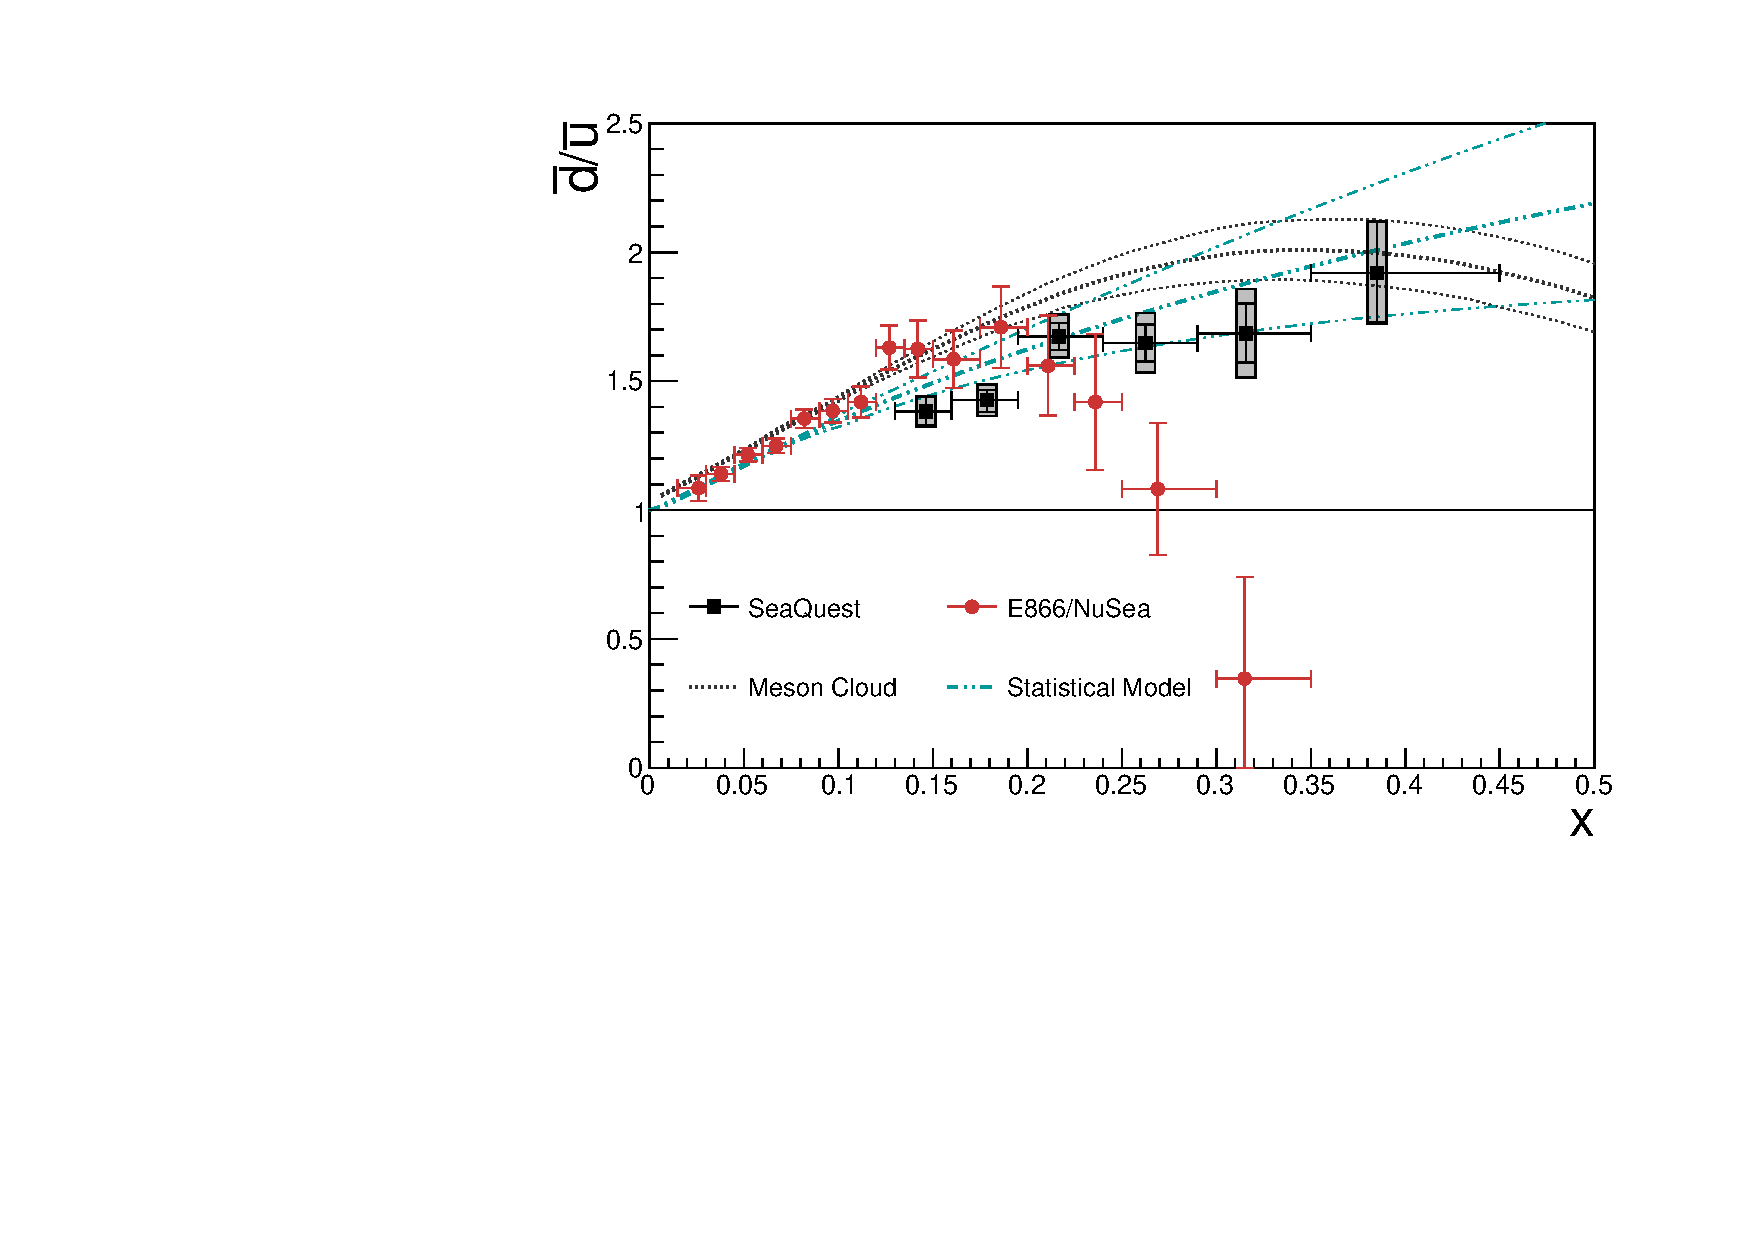
\includegraphics[width=\linewidth]{E906_E866_dbarubar_model.pdf}
	\end{subfigure}
	\begin{subfigure}{0.45\linewidth}
		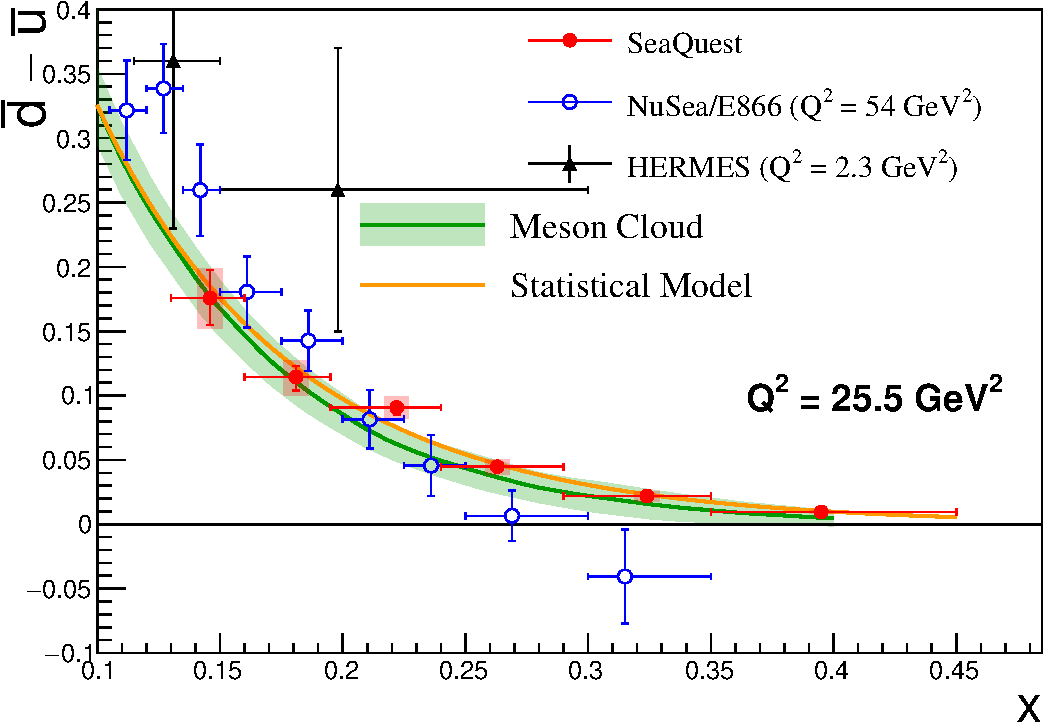
\includegraphics[width=\linewidth]{dbub_diff_with_model.pdf}
	\end{subfigure}
	\caption{The extracted $\bar{d}(x)/\bar{u}(x)$ (left) and $\bar{d}(x)-\bar{u}(x)$ (right)
		from the measured $\sigma_{pd}/2\sigma_{pp}$ Drell-Yan cross section ratio
		from SeaQuest (black square), E866~\cite{towell2001} (red circles), and HERMES~\cite{ackerstaff1998} (blue triangles).
		The extracted ratios are compared with predictions from the meson cloud model~\cite{alberg2022} and the statistical model~\cite{soffer2019}.
		%The error bands on the PDFs correspond to their \SI{68}{\percent} confidence level.
	}
	\label{fig:e906_e866_dbarubar_model}
\end{figure*}
\end{comment}
\end{document}

